\section{Assignment 1 images}

\label{app:confusion_matrix}
\begin{figure}[H]
\centering
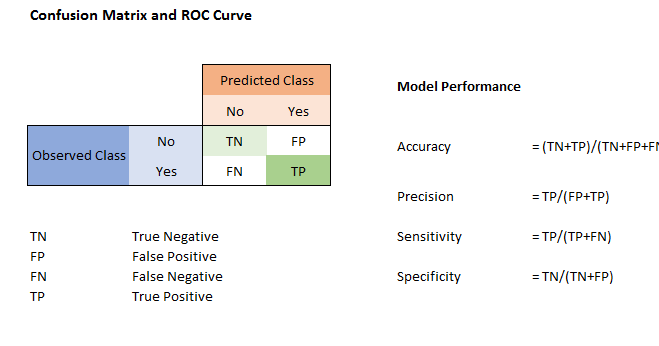
\includegraphics[scale=0.55]{Graphics/Assignment1/ConfusionMatrix.png}
\caption{Confusion Matrix}
\label{fig:confusion_Matrix}
\end{figure}

\subtitle{LDA coefficients results}
\begin{figure}[H]
\centering
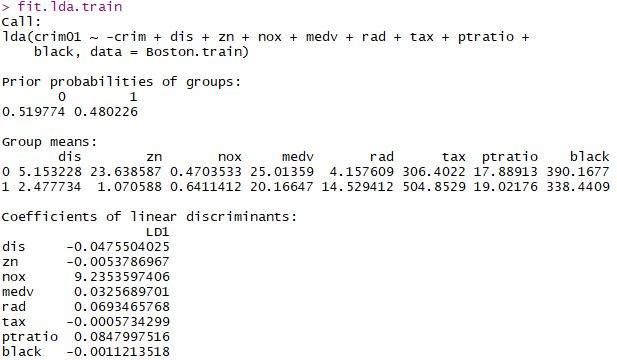
\includegraphics[scale=0.55]{Graphics/Assignment1/LDACoefficients_005.JPG}
\caption{Coefficients for significance level 5\%}
\label{fig:coefficients_method_005}
\end{figure}

\begin{figure}[H]
\centering
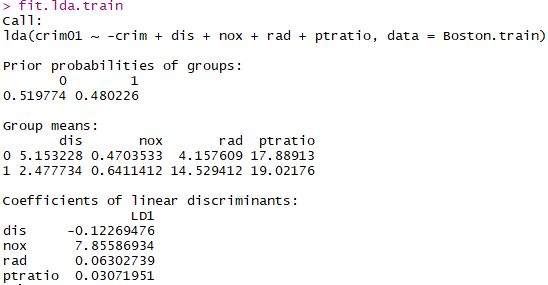
\includegraphics[scale=0.55]{Graphics/Assignment1/LDACoefficients_001.JPG}
\caption{Coefficients for significance level 1\%}
\label{fig:coefficients_method_001}
\end{figure}

\begin{figure}[H]
\centering
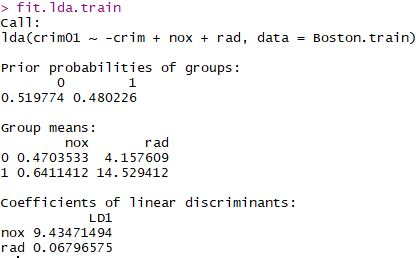
\includegraphics[scale=0.55]{Graphics/Assignment1/LDACoefficients_0001.JPG}
\caption{Coefficients for significance level 0.1\%}
\label{fig:coefficients_method_0001}
\end{figure}


\section{Assignment 3 images}
%--------------- Renoir Image -------------------------
\begin{figure}[H]
    \centering
    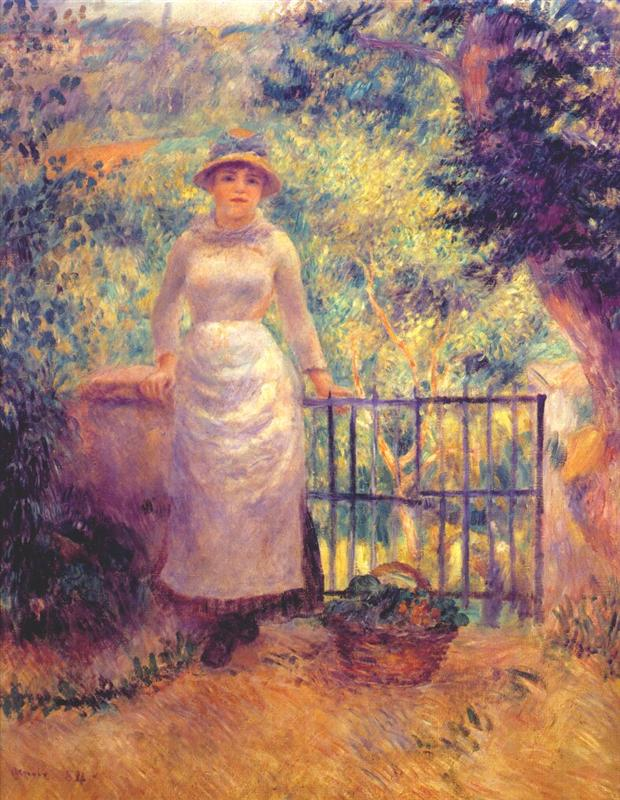
\includegraphics[scale=0.3]{Graphics/Assignment3/renoir.png}
    \caption{Pierre-Auguste Renoir: Aline at the gate.}
    \label{fig:renoir}
\end{figure}
%--------------- Outlier Image -------------------------

\begin{figure}[H]
    \centering
    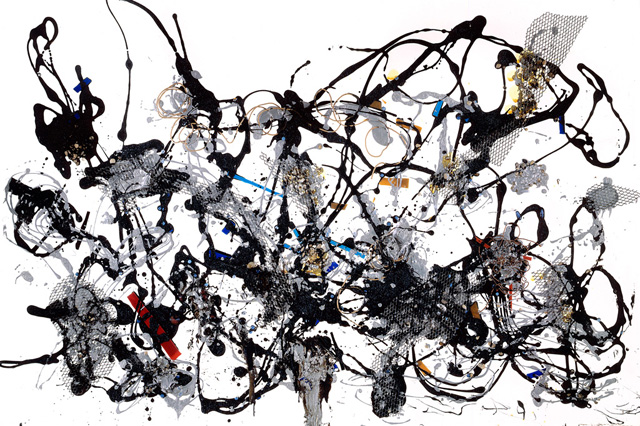
\includegraphics[scale=0.5]{Graphics/Assignment3/outlier.png}
    \caption{Jackson Pollock: Number 29.}
    \label{fig:outlier}
\end{figure}

%--------------- Manet Image -------------------------
\begin{figure}[H]
    \centering
    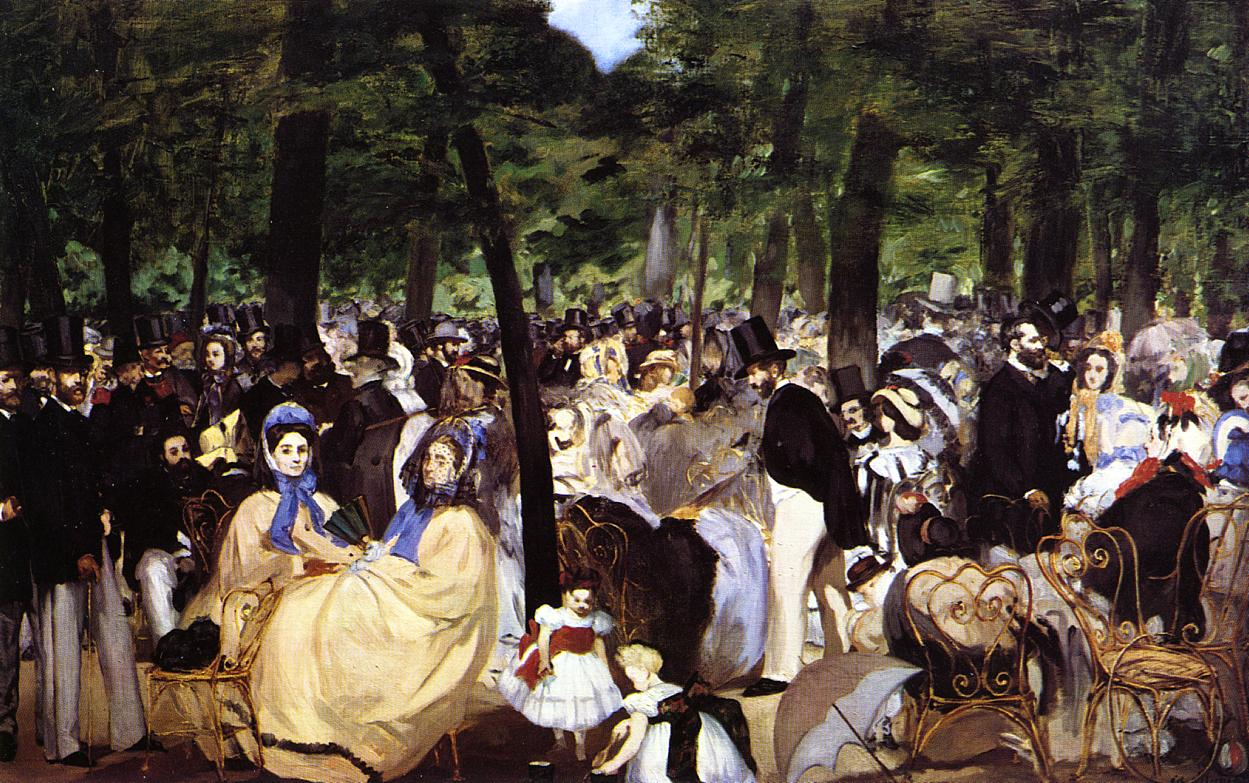
\includegraphics[scale=0.3]{Graphics/Assignment3/manet.png}
    \caption{Édouard Manet: Music in the Tuileries.}
    \label{fig:manet}
\end{figure}


%--------------- Degas Image -------------------------

\begin{figure}[H]
    \centering
    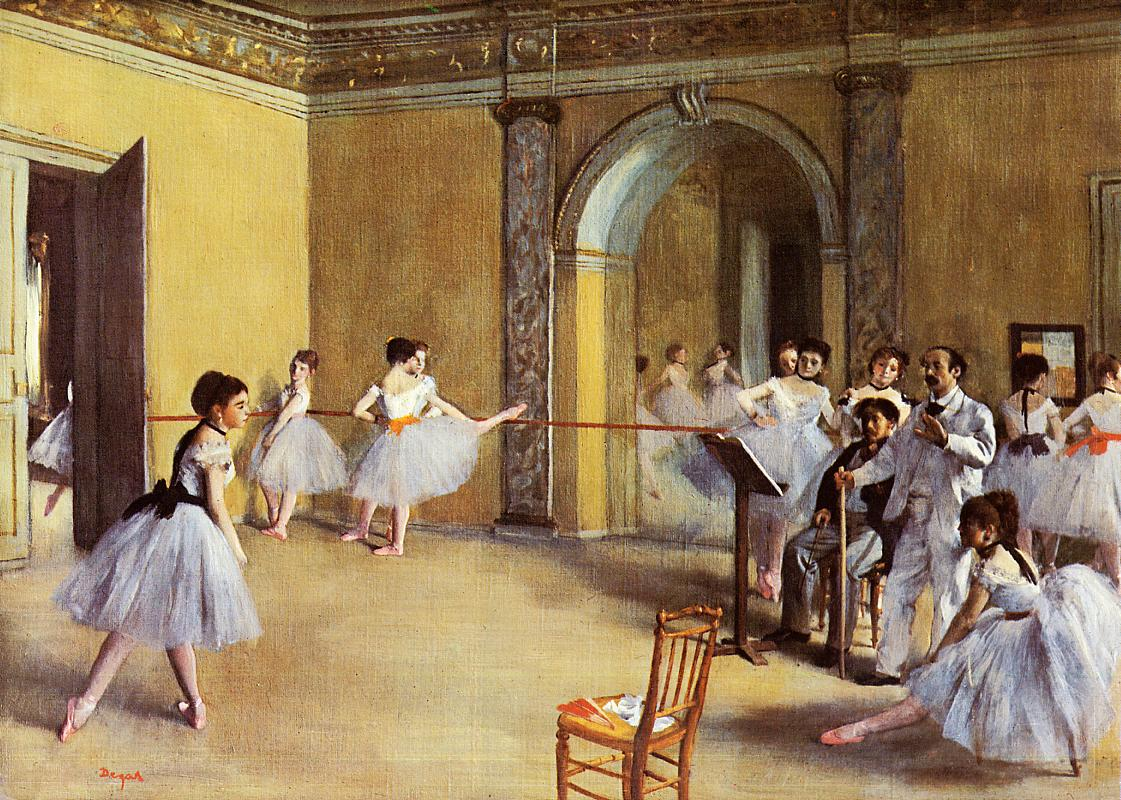
\includegraphics[scale=0.3]{Graphics/Assignment3/degas.png}
    \caption{Edgar Degas: Dance Class at the Opera.}
    \label{fig:degas}
\end{figure}

%--------------- VGG16 model Image -------------------------

\begin{figure}[H]
    \centering
    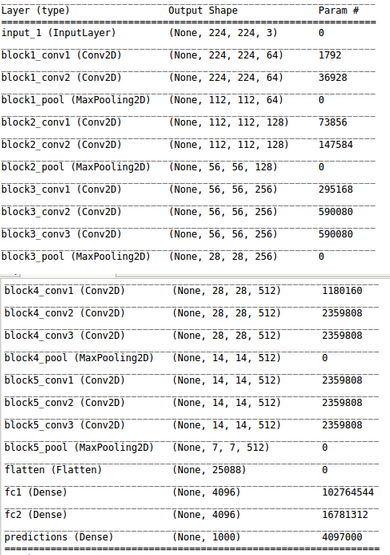
\includegraphics[scale=0.7]{Graphics/Assignment3/VGG16_model_image.png}
    \caption{VGG16 model with 1000 classes as output.}
    \label{fig:imagenet_vgg16}
\end{figure}

%--------------- Custom VGG16 model Image -------------------------

\begin{figure}[H]
    \centering
    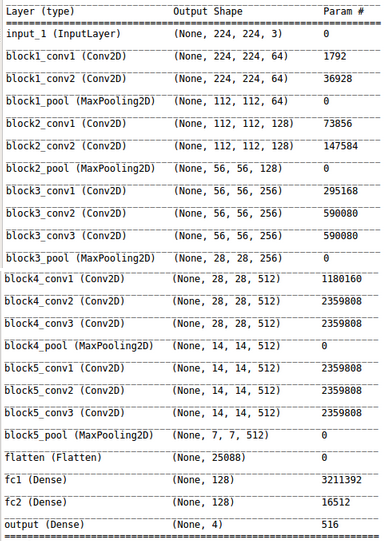
\includegraphics[scale=0.7]{Graphics/Assignment3/custom_model_image.png}
    \caption{Custom VGG16 model with 4 classes as output.}
    \label{fig:custom_vgg16}
\end{figure}

\section{Assignment 3 code}

%------------------ Fetch image code ----------------------
\begin{lstlisting}[frame=single, language=Bash, label={code:fetch_images}, caption={Code to fetch images from Wikiart for specific artists, in this case Manet.}]
    curl -s "https://www.wikiart.org/en/App/Painting/PaintingsByArtist?artistUrl=edouard-manet&json=2" | jq -r 'map(.image) | join("\n")' | sed '' | xargs -P 10 -n 1 curl -s -O
\end{lstlisting}

%------------------ Load data for preprocessing ---------------
\begin{lstlisting}[frame=single, language=Python, label={code:load_data}, caption={Code to load data for preprocessing.}]
    for dataset in data_dir_list:
	    img_list=os.listdir(data_path+'/'+ dataset)
    	for img in img_list:
    		img_path = data_path + '/'+ dataset + '/'+ img 
    		img = image.load_img(img_path, target_size=(224, 224))
    		x = image.img_to_array(img)
    		x = np.expand_dims(x, axis=0)
    		x = preprocess_input(x)
    		img_data_list.append(x)
\end{lstlisting}


%------------------- Shuffle and split into training and test --------------------
\begin{lstlisting}[frame=single, language=Python, label={code:shuffle_and_split_data}, caption={Code to shuffle and split the data to 80\% training and 20\% test.}]
#Shuffle the dataset
x,y = shuffle(img_data,Y, random_state=2)

# Split the dataset
X_train, X_test, y_train, y_test = train_test_split(x, y, test_size=0.2, random_state=2)
\end{lstlisting}

\begin{lstlisting}[frame=single, language=Python, label={code:model_creation_and_training}, caption={Code to load VGG16 pre-trained on ImageNet and doing transfer learning.}]
# Adjust the image input to 224, 224 and 3 channels
image_input = Input(shape=(224, 224, 3))

# VGG16 model
model = VGG16(input_tensor=image_input, include_top=True,weights='imagenet')

# Get VGG16's block5_pool layer and take its output
last_layer = model.get_layer('block5_pool').output
# Feed the output of block5_pool to the Flatten layer
x= Flatten(name='flatten')(last_layer)
# Create two fully connected layers with 128 neurons each, using RELU activation
x = Dense(128, activation='relu', name='fc1')(x)
x = Dense(128, activation='relu', name='fc2')(x)
# Create a output layer, using softmax classification
out = Dense(num_classes, activation='softmax', name='output')(x)
# Assign the new model to a variable
custom_vgg_model2 = Model(image_input, out)

# Freeze all the layers except the dense layers that was created above
for layer in custom_vgg_model2.layers[:-3]:
	layer.trainable = False

# Compile the new model architecture
custom_vgg_model2.compile(loss='categorical_crossentropy',optimizer='adadelta',metrics=['accuracy'])

# Time it
t=time.time()
# Train the model for 20 epochs using a batch size of 4
hist = custom_vgg_model2.fit(X_train, y_train, batch_size=4, epochs=20, verbose=1, validation_data=(X_test, y_test))
print('Training time: %s' % (t - time.time()))
# Test the model using accuracy as a metric
(loss, accuracy) = custom_vgg_model2.evaluate(X_test, y_test, batch_size=10, verbose=1)
print("[INFO] loss={:.4f}, accuracy: {:.4f}%".format(loss,accuracy * 100))
\end{lstlisting}



